\chapter{Specifica dei Requisiti Software}

\section{Attori del Sistema}

Considerando il tipo di sistema in sviluppo --- una piattaforma per la gestione collaborativa di progetti software --- il background tecnico degli utenti sarà relativamente omogeneo. La maggior parte saranno sviluppatori, ad eccezione dei team leader, che potrebbero avere competenze tecniche meno avanzate.

Possiamo quindi definire due classi di utenti:

\begin{itemize}
    \item \textbf{Utente standard}: sviluppatori software, tester e figure tecniche operative.
    \item \textbf{Utente amministratore}: team leader, manager, project manager e altri stakeholders con responsabilità di coordinamento e supervisione del progetto.
\end{itemize}
\renewcommand{\arraystretch}{1.5}
\setlength{\tabcolsep}{8pt}

\definecolor{headersBlue}{HTML}{003366}

\begin{longtable}{|p{3.5cm}|p{5.5cm}|p{5.5cm}|}
\caption{Caratterizzazione degli attori}
\label{tab:caratterizzazione-attori} \\

\hline
\rowcolor{headersBlue!30}
\textbf{Attore} & \textbf{Utente Standard} (Sviluppatore, Tester) & \textbf{Utente Amministratore} (Team Leader, Project Manager) \\
\hline
\endfirsthead

\hline
\rowcolor{headersBlue!30}
\textbf{Attore} & \textbf{Utente Standard} (Sviluppatore, Tester) & \textbf{Utente Amministratore} (Team Leader, Project Manager) \\
\hline
\endhead

\hline
\textbf{Ruoli e Responsabilità} &
Segnalazione issues, assegnazione task, sviluppo codice, esecuzione e supervisione dei test, documentazione tecnica, collaborazione su task assegnati &
Coordinamento team, monitoraggio avanzamento, gestione priorità, reporting, supervisione generale del progetto \\
\hline

\textbf{Competenze Tecniche} &
Conoscenza avanzata di linguaggi di programmazione, testing, version control, metodologie di sviluppo &
Conoscenze tecniche di base/intermedie, competenze gestionali, pianificazione progetti, gestione risorse \\
\hline

\textbf{Frequenza e Modalità d'Uso} &
Utilizzo quotidiano, accesso continuo durante orario lavorativo, interazione con task e repository &
Utilizzo regolare (giornaliero/settimanale), focus su dashboard, reportistica e gestione team \\
\hline

\textbf{Obiettivi} &
Completare task assegnati, collaborare con il team, mantenere qualità del codice, rispettare le deadline &
Garantire rispetto timeline, allocare risorse efficacemente, monitorare performance del team, gestire rischi \\
\hline

\textbf{Privilegi di Accesso} &
Creazione, lettura/scrittura su task, accesso ai repository del progetto, creazione issue e commenti &
Accesso completo al progetto, creazione, modifica, eliminazione task, gestione utenti, configurazione progetto, accesso a statistiche e reportistica avanzata \\
\hline

\end{longtable}

\section{Requisiti Non Funzionali}

Il sistema sarà composto da due moduli principali: un \textbf{frontend} e un \textbf{backend}.  
Il frontend sarà una \textit{Single Page Application (SPA)}, sviluppata presumibilmente tramite framework come \textbf{Angular} o \textbf{React}, mentre il backend sarà implementato in \textbf{Java}, utilizzando tecnologie come \textbf{Spring}, \textbf{Hibernate} o \textbf{Jakarta EE}.

\subsection{Requisiti del Prodotto}

\subsubsection{Usabilità}
\begin{itemize}
    \item Il sistema dovrà essere facile da usare ed intuitivo.
    \item Il frontend dovrà essere \textbf{responsive}, garantendo un'esperienza ottimale sia su dispositivi desktop che mobili.
    \item Un utente istruito deve poter completare un'attività primaria senza necessità di assistenza.
    \item Un amministratore con formazione adeguata deve poter registrare un nuovo utente in meno di 2 minuti.
    \item Gli elementi dell'interfaccia e i comportamenti (es. animazioni) devono essere coerenti nelle varie pagine per colori, dimensioni e tempi.
    \item I nuovi utenti devono poter completare almeno il 90\% dei task basilari (creazione, aggiornamento, ricerca, filtraggio, ordinamento delle issues) dopo 30 minuti di addestramento.
    \item I messaggi di errore devono essere chiari e fornire indicazioni sulle azioni correttive.
    \item Le funzionalità principali devono essere individuabili senza istruzioni.
    \item I titoli devono rispettare un limite massimo di caratteri per garantire la leggibilità completa delle issues.
    \item Ogni funzionalità principale deve essere raggiungibile con un massimo di 5 click dalla homepage.
\end{itemize}

\subsubsection{Efficienza}
\begin{itemize}
    \item Il sistema deve essere performante, con un'esperienza coerente tra versione desktop e mobile.
    \item Deve essere possibile caricare immagini fino a 5 MB senza compromettere le prestazioni.
    \item Il tempo di risposta per le operazioni basilari non deve superare 1 secondo.
\end{itemize}

\subsubsection{Affidabilità}
\begin{itemize}
    \item Il sistema deve garantire un \textbf{uptime del 99.5\%} su base mensile durante gli orari lavorativi.
\end{itemize}

\subsubsection{Sicurezza}
\begin{itemize}
    \item Gli utenti devono cambiare la password temporanea fornita al primo login.
    \item Le password devono essere sottoposte ad algoritmi di hashing prima del salvataggio.
    \item Le sessioni devono essere gestite tramite \textbf{JSON Web Tokens (JWT)} con validazione.
    \item Il sistema deve essere protetto da attacchi \textbf{CSRF}, \textbf{XSS} e \textbf{SQL Injection}.
    \item Le password devono rispettare criteri minimi di complessità (minimo 8 caratteri, almeno una maiuscola, un numero e un carattere speciale).
\end{itemize}

\subsubsection{Manutenibilità}
\begin{itemize}
    \item L'architettura deve essere modulare per facilitare aggiornamenti e manutenzione.
    \item Deve essere implementato un sistema di \textbf{log strutturato} con livelli di severità.
    \item La documentazione del codice deve seguire gli standard \textbf{JavaDoc} (backend) e \textbf{JSDoc}/\textbf{TSDoc} (frontend).
    \item Le dipendenze di terze parti devono poter essere aggiornate senza modifiche strutturali al codice.
\end{itemize}

\subsection{Requisiti Organizzativi}

\subsubsection{Ambientali}
\begin{itemize}
    \item Il sistema dovrà essere ospitato su piattaforme di \textbf{cloud computing}, garantendo accesso continuo e universale.
    \item Il sistema deve essere \textbf{containerizzato} tramite \textbf{Docker}.
    \item Deve poter gestire almeno 200 utenti concorrenti senza degrado percepibile delle prestazioni.
\end{itemize}

\subsubsection{Operativi}
\begin{itemize}
    \item Browser supportati: ultime due versioni stabili di \textbf{Chrome}, \textbf{Firefox}, \textbf{Edge} e \textbf{Safari}.
\end{itemize}

\subsubsection{Di Sviluppo}
\begin{itemize}
    \item L'intera codebase deve essere versionata tramite \textbf{Git}.
    \item Ogni \textit{pull request} deve essere approvata da almeno un altro sviluppatore.
    \item La qualità del codice deve essere verificata automaticamente tramite \textbf{SonarQube}.
    \item Gli sviluppatori devono utilizzare strumenti di analisi statica e \textit{linter} integrati nel proprio IDE.
\end{itemize}


\section{Modellazione dei Casi d'uso}

\begin{figure}[H]
    \centering
    
\includegraphics[width=\textwidth]{diagrams/usecase-diagram.pdf}
    \caption{Diagramma dei casi d'uso principali di BugBoard26.}
\end{figure}

\newpage

\section{Casi d'uso Significativi}
I casi d'uso presentati in questa sezione rappresentano alcune delle interazioni principali che caratterizzano il funzionamento del sistema BugBoard26.

La metodologia di documentazione adottata segue le linee guida contenute in \textit{A Practical Style Guide and Templates Repository for Writing Effective Use Cases} \cite{Wei2022}, che fornisce, citando gli autori, \textit{An opinionated style guide for use case writing} \cite{Washingtonwei2023} attraverso il formalismo di Alistair Cockburn \cite{cockburn-use-cases}. Questo approccio ci consente di descrivere in modo sistematico e coerente:

\begin{itemize}
    \item L'obiettivo primario di ciascun caso d'uso dal punto di vista dell'attore
    \item Il flusso principale degli eventi e le relative condizioni di attivazione
    \item Gli eventuali flussi alternativi
    \item Le precondizioni necessarie e le postcondizioni attese
\end{itemize}

Per ogni caso d'uso significativo, forniamo una descrizione strutturata secondo il modello di Cockburn e una tabella delle proprietà rilevanti. Questo livello di dettaglio è necessario per garantire che le funzionalità chiave del sistema siano comprese in modo inequivocabile da tutte le parti interessate, dagli stakeholders agli sviluppatori.

Di seguito riportiamo i casi d'uso selezionati, che costituiscono alcune delle funzionalità \textit{core} di BugBoard26 e rappresentano i principali flussi di interazione con il sistema.

\subsection{UC1 - Creazione di una issue}
\begin{center}
    \begin{longtable}{|p{4cm}|p{11cm}|}
    \hline
    \textbf{ID - Nome dello UC} & 1 - Creazione di una issue \cite{uc1-figma} \\
    \hline
    \textbf{Data di creazione} & 11/10/2025 \\
    \hline
    \textbf{Attore primario} & Utente \\
    \hline
    \textbf{Trigger} & L'utente indica di voler creare una nuova issue \\
    \hline
    \textbf{Descrizione} & L'utente ha trovato un problema e intende aprire una nuova issue per tenere traccia di esso. \\
    \hline
    \textbf{Precondizioni} & \textbf{PRE-1.} L'utente è stato registrato da un amministratore ed ha effettuato correttamente l'autenticazione \newline
    \textbf{PRE-2.} Il sistema ha caricato la pagina di riepilogo delle issues \\
    \hline
    \textbf{Postcondizioni} & \textbf{POST-1.} La nuova issue è salvata nel sistema \newline
    \textbf{POST-2.} La nuova issue è visibile nella vista di riepilogo delle issue \\
    \hline
    \textbf{Scenario di successo} & 1. L'utente indica di voler segnalare una nuova issue (M1) \newline
    2. Il sistema apre la modale di creazione di una nuova issue (M2) \newline
    3. L'utente inserisce il titolo della issue (M3) \newline
    4. L'utente indica i dettagli della issue nella descrizione (M4) \newline
    4a. [Opzionale] L'utente sceglie una priorità per la issue \newline
    4b. [Opzionale] L'utente può allegare un'immagine \newline
    4c. [Opzionale] L'utente sceglie un tipo per la issue \newline
    5. L'utente segnala di aver terminato l'inserimento dei dati richiesti (M5) \newline
    6. Il sistema valida i dati inseriti dall'utente \newline
    7. Il sistema salva la nuova issue \newline
    8. Il sistema mostra un messaggio di successo (M6) \\
    \hline

    \multicolumn{2}{r}{\small Continua nella pagina successiva} \\
    \textbf{Estensioni} & \textbf{4a. Scelta della priorità per la issue:} \newline
    4a1. L'utente clicca sul menù “priorità” (M9) \newline
    4a2. Il sistema apre un menù con le possibili priorità (M10) \newline
    4a3. L'utente sceglie una tra le alternative (M11) \newline
    4a4. Il sistema mostra l'alternativa scelta (M12) \newline
    4a5. Il flusso ritorna al termine del punto 4 dello scenario di successo \newline

    \textbf{4b. Caricamento di un'immagine:} \newline
    4b1. L'utente clicca sul bottone per caricare un'immagine (M13) \newline
    4b2. Il sistema apre il file explorer (M14) \newline
    4b3. L'utente seleziona un'immagine dal proprio dispositivo (M15, M16) \newline
    4b4. Il sistema valida il formato e la dimensione dell'immagine \newline
    4b5. Il sistema sostituisce l'icona di “allega” con un messaggio di successo (\checkmark) e aggiunge un bottone di eliminazione accanto alla label “immagine”(M17) \newline
    4b7. Il flusso torna al termine del punto 4a dello scenario di successo \newline

    \textbf{4b3a. L'utente annulla il caricamento dell'immagine:} \newline
    4b3a1. L'utente clicca sul bottone “annulla” \newline
    4b3a2. Il flusso ritorna al termine del punto 4 dello scenario di successo \newline

    \textbf{4b4a. Errore di validazione dell'immagine:} \newline
    4b4a1. Il sistema mostra un messaggio di errore e invita l'utente a riprovare (M18) \newline
    4b4a2. Il flusso ritorna al termine del punto 4 dello scenario di successo \newline

    \textbf{4b6a. Eliminazione dell'immagine allegata:} \newline
    4b6a1. L'utente clicca sul bottone di eliminazione \newline
    4b6a2. Il sistema elimina l'immagine allegata \newline
    4b6a3. Il sistema sostituisce l'icona di successo (\checkmark) con il bottone “allega” e rimuove il bottone di eliminazione \newline
    4b6a4. Il flusso ritorna al termine del punto 4 dello scenario di successo \\
    \hline
    \multicolumn{2}{r}{\small Continua nella pagina successiva}
    \end{longtable}


    \begin{longtable}{|p{4cm}|p{11cm}|}
    \hline
    \textbf{Estensioni} & 
    \textbf{4c. Scelta del tipo di issue:} \newline
    4c1. L'utente clicca sul menù “tipo” (M19) \newline
    4c2. Il sistema apre il menù con i vari tipi di issues (M20) \newline
    4c3. L'utente sceglie un tipo di issue (M21) \newline
    4c4. Il sistema mostra il tipo scelto (M22) \newline
    4c5. Il flusso ritorna al termine del punto 4 dello scenario di successo \newline

    \textbf{6a. Errore nella validazione dell'input (titolo):} \newline
    6a1. L'utente inserisce un titolo non valido \newline
    6a2. Il sistema evidenzia il campo del titolo e mostra un messaggio all'utente, segnalando la non validità del titolo scelto (M7) \newline
    6a3. L'utente modifica il titolo, inserendone uno corretto (M3) \newline
    6a4. Il flusso ritorna al punto 4 dello scenario di successo \newline

    \textbf{6b. Errore nella validazione dell'input (descrizione):} \newline
    6b1. L'utente inserisce una descrizione non valida \newline
    6b2. Il sistema evidenzia il campo della descrizione e mostra un messaggio all'utente, segnalando la non validità della descrizione scelta (M8) \newline
    6b3. L'utente inserisce una descrizione valida (M4) \newline
    6b4. Il flusso ritorna al punto 5 nello scenario di successo \newline

    \textbf{7a. Errore nel salvataggio della issue:} \newline
    7a1. Il sistema riscontra un errore durante il salvataggio della issue \newline
    7a2. Il sistema mostra uno specifico messaggio di errore, invitando l'utente a riprovare (M23) \newline
    7a3. Il flusso ritorna al termine del punto 4 nello scenario di successo \\
    \hline
    \textbf{Priorità} & Alta \\
    \hline
    \textbf{Frequenza d'uso} & Presumibilmente tutti gli utenti, tra 1 e 5 volte al giorno per utente \\
    \hline
    \textbf{Informazioni associate} & Mostrato nella tabella ~\ref{tab:uc1-proprieta} \\
    \hline
\end{longtable}

\newpage
    \begin{table}[H]
    \centering
    \renewcommand{\arraystretch}{1.5}
    \begin{tabular}{|p{4cm}|p{4cm}|p{6cm}|}
        \hline
        \textbf{Nome della proprietà} & \textbf{Tipo} & \textbf{Regole di validazione} \\
        \hline
        Titolo & String & Obbligatorio, compreso tra 10 e 100 caratteri \\
        \hline
        Descrizione & String & Obbligatorio, compreso tra 30 e 30000 caratteri \\
        \hline
        Priorità & String & Facoltativo, valori possibili: \newline
        - Lowest \newline
        - Low \newline
        - Medium \newline
        - High \newline
        - Highest \\
        \hline
        Immagine & File (image) & Facoltativo, dimensione massima: 5Mb \\
        \hline
        Tipo & String & Facoltativo, valori possibili: \newline
        - Question \newline
        - Bug \newline
        - Documentation \newline
        - Feature \\
        \hline
    \end{tabular}
    \caption{Regole di validazione delle proprietà}
    \label{tab:uc1-proprieta}
\end{table}
\newpage
\end{center}

\subsubsection{AC1 - Creazione di una issue}
\begin{figure}[H]
  \centering
  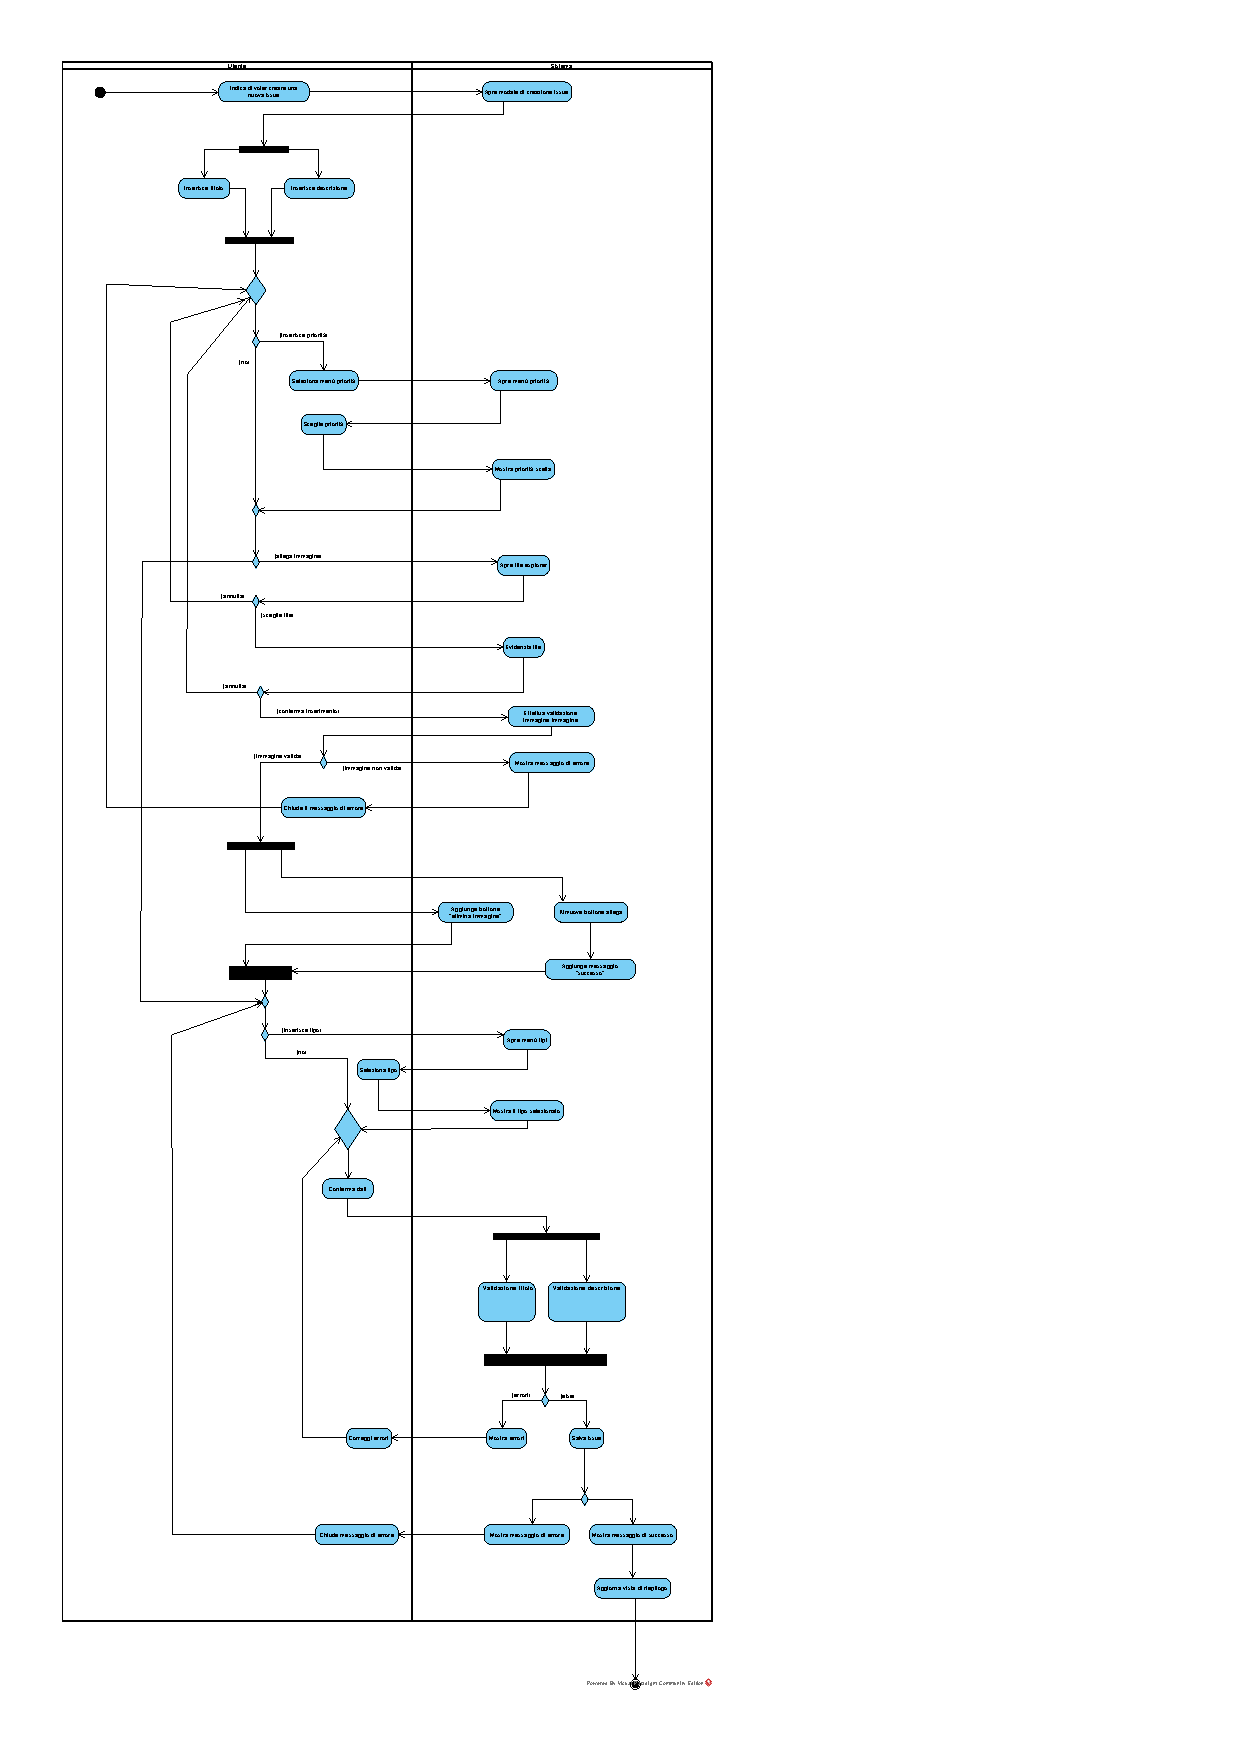
\includegraphics[width=\linewidth,height=0.75\textheight,keepaspectratio]{media/diagrams/AC-CreateIssue.pdf}
  \caption{Diagramma d'attività della creazione di una nuova issue}
\end{figure}


\subsection{UC2 - Associazione di etichette personalizzate}
\subsubsection{Descrizione Strutturata (Formalismo di A. Cockburn)}
\begin{center}
    % UC-4 Ordinamenti — Template di Cockburn (LONGTABLE con griglia completa)
% Include con: % UC-4 Ordinamenti — Template di Cockburn (LONGTABLE con griglia completa)
% Include con: % UC-4 Ordinamenti — Template di Cockburn (LONGTABLE con griglia completa)
% Include con: \input{UC3 - Cockburn.txt}
% Compilazione: XeLaTeX o LuaLaTeX consigliati (oppure pdfLaTeX con \usepackage[utf8]{inputenc})
% Preambolo richiesto:
% \usepackage{longtable}
% \usepackage{array}
% \usepackage{enumitem} % per itemize/enumerate compatti
\renewcommand{\arraystretch}{1.25}
\setlength{\tabcolsep}{8pt}

\begin{longtable}{|p{4cm}|p{11cm}|}
\caption{UC-3 Ordinamenti -- Template di Cockburn}\label{tab:uc3-cockburn}\\
\hline
\textbf{Campo} & \textbf{Valore} \\ \hline
\endfirsthead

\hline
\textbf{Campo} & \textbf{Valore} \\ \hline
\endhead
\hline
\multicolumn{2}{r}{\small Continua nella pagina successiva} \\
\endfoot
\hline
\endlastfoot

\textbf{ID - Nome dello UC} & 3 - Ordinamento \cite{uc3-figma} \\ \hline
\textbf{Data di creazione} & 14/10/2025 \\ \hline
\textbf{Attore primario} & Utente \\ \hline
\textbf{Trigger} & L'utente indica di voler ordinare l'elenco delle issues. \\ \hline
\textbf{Descrizione} & L'utente vuole ordinare le issues presenti nell'elenco tramite un criterio specifico. \\ \hline

\textbf{Precondizioni} &
\begin{minipage}[t]{\linewidth}\raggedright
\begin{itemize}[leftmargin=*,nosep]
\item PRE-1. L'utente è stato registrato da un amministratore ed ha effettuato correttamente l'autenticazione.
\item PRE-2. Il sistema ha caricato la pagina di riepilogo delle issues.
\end{itemize}
\end{minipage} \\ \hline

\textbf{Postcondizioni} & L'elenco delle issues è riordinato. \\ \hline

\textbf{Scenario di successo} &
\begin{minipage}[t]{\linewidth}\raggedright
\begin{enumerate}[leftmargin=*,nosep]
\item L'utente visualizza la tabella contenente le issues con le relative colonne.
\item L'utente clicca sull'intestazione di una colonna (es. stato, priorità, data creazione) per applicare un ordinamento.
\item Il sistema riordina la tabella in base ai valori della colonna selezionata e mostra un indicatore visivo della direzione dell'ordinamento (es. \uparrow o \downarrow).
\item \textit{[Opzionale]} L'utente clicca su ulteriori intestazioni di colonna per definire un ordinamento secondario o terziario.
\item \textit{[Opzionale]} Se l'utente clicca nuovamente su una colonna già ordinata, il sistema inverte la direzione dell'ordinamento o ripristina l'ordine predefinito.
\item Il sistema mostra la tabella aggiornata e, se previsto, memorizza i criteri di ordinamento nella sessione o nell'URL.
\end{enumerate}
\end{minipage} \\ \hline

\textbf{Estensioni} &
\begin{minipage}[t]{\linewidth}\raggedright
\textbf{3a. Ordinamento crescente/decrescente}\\
3a1. L'utente clicca una seconda volta sulla stessa intestazione di colonna.\\
3a2. Il sistema inverte la direzione dell'ordinamento (da crescente a decrescente o viceversa).\\
3a3. Il sistema aggiorna l'indicatore visivo (freccia \uparrow/\downarrow \) ) e ricarica la tabella.\\
3a4. Il flusso ritorna al termine del punto 3 dello scenario di successo.\\[0.6em]

\textbf{4a. Ordinamento secondario o multiplo}\\
4a1. L'utente clicca su un'altra intestazione di colonna diversa da quella attiva.\\
4a2. Il sistema imposta un secondo livello di ordinamento, mantenendo la gerarchia (es. priority → stato).\\
4a3. Il sistema aggiorna la tabella e mostra indicatori visivi multipli per le colonne coinvolte.\\
4a4. Il flusso ritorna al termine del punto 4 dello scenario di successo.\\[0.6em]

\textbf{4b. Rimozione di un ordinamento attivo}\\
4b1. L'utente clicca nuovamente su una colonna ordinata fino a tornare alla condizione “nessun ordine”.\\
4b2. Il sistema rimuove l'indicatore visivo e ripristina l'ordinamento predefinito.\\
4b3. Il flusso ritorna al termine del punto 3 dello scenario di successo.\\[0.6em]

\textbf{6a. Persistenza dell'ordinamento}\\
6a1. Il sistema salva automaticamente le informazioni sull'ordinamento corrente nella sessione o nell'URL.\\
6a2. Quando la pagina viene ricaricata o condivisa, l'ordinamento precedente viene ripristinato.\\
6a3. Il flusso prosegue dal punto 6 dello scenario di successo.\\[0.6em]

\textbf{6b. Ordinamento su colonna non ordinabile}\\
6b1. L'utente clicca su una colonna che non supporta l'ordinamento (es. colonna tag).\\
6b2. Il sistema ignora il click senza modificare la tabella.\\
6b3. Il flusso ritorna al punto 2 dello scenario di successo.
\end{minipage} \\ \hline

\textbf{Priorità} & Media \\ \hline
\textbf{Frequenza d'uso} & Tutti gli utenti, tra 1 e 3 volte al giorno per utente \\ \hline
\textbf{Informazioni associate} & Mostrato nella Tabella~\ref{tab:uc3-proprieta} \\ \hline

\end{longtable}
% Compilazione: XeLaTeX o LuaLaTeX consigliati (oppure pdfLaTeX con \usepackage[utf8]{inputenc})
% Preambolo richiesto:
% \usepackage{longtable}
% \usepackage{array}
% \usepackage{enumitem} % per itemize/enumerate compatti
\renewcommand{\arraystretch}{1.25}
\setlength{\tabcolsep}{8pt}

\begin{longtable}{|p{4cm}|p{11cm}|}
\caption{UC-3 Ordinamenti -- Template di Cockburn}\label{tab:uc3-cockburn}\\
\hline
\textbf{Campo} & \textbf{Valore} \\ \hline
\endfirsthead

\hline
\textbf{Campo} & \textbf{Valore} \\ \hline
\endhead
\hline
\multicolumn{2}{r}{\small Continua nella pagina successiva} \\
\endfoot
\hline
\endlastfoot

\textbf{ID - Nome dello UC} & 3 - Ordinamento \cite{uc3-figma} \\ \hline
\textbf{Data di creazione} & 14/10/2025 \\ \hline
\textbf{Attore primario} & Utente \\ \hline
\textbf{Trigger} & L'utente indica di voler ordinare l'elenco delle issues. \\ \hline
\textbf{Descrizione} & L'utente vuole ordinare le issues presenti nell'elenco tramite un criterio specifico. \\ \hline

\textbf{Precondizioni} &
\begin{minipage}[t]{\linewidth}\raggedright
\begin{itemize}[leftmargin=*,nosep]
\item PRE-1. L'utente è stato registrato da un amministratore ed ha effettuato correttamente l'autenticazione.
\item PRE-2. Il sistema ha caricato la pagina di riepilogo delle issues.
\end{itemize}
\end{minipage} \\ \hline

\textbf{Postcondizioni} & L'elenco delle issues è riordinato. \\ \hline

\textbf{Scenario di successo} &
\begin{minipage}[t]{\linewidth}\raggedright
\begin{enumerate}[leftmargin=*,nosep]
\item L'utente visualizza la tabella contenente le issues con le relative colonne.
\item L'utente clicca sull'intestazione di una colonna (es. stato, priorità, data creazione) per applicare un ordinamento.
\item Il sistema riordina la tabella in base ai valori della colonna selezionata e mostra un indicatore visivo della direzione dell'ordinamento (es. \uparrow o \downarrow).
\item \textit{[Opzionale]} L'utente clicca su ulteriori intestazioni di colonna per definire un ordinamento secondario o terziario.
\item \textit{[Opzionale]} Se l'utente clicca nuovamente su una colonna già ordinata, il sistema inverte la direzione dell'ordinamento o ripristina l'ordine predefinito.
\item Il sistema mostra la tabella aggiornata e, se previsto, memorizza i criteri di ordinamento nella sessione o nell'URL.
\end{enumerate}
\end{minipage} \\ \hline

\textbf{Estensioni} &
\begin{minipage}[t]{\linewidth}\raggedright
\textbf{3a. Ordinamento crescente/decrescente}\\
3a1. L'utente clicca una seconda volta sulla stessa intestazione di colonna.\\
3a2. Il sistema inverte la direzione dell'ordinamento (da crescente a decrescente o viceversa).\\
3a3. Il sistema aggiorna l'indicatore visivo (freccia \uparrow/\downarrow \) ) e ricarica la tabella.\\
3a4. Il flusso ritorna al termine del punto 3 dello scenario di successo.\\[0.6em]

\textbf{4a. Ordinamento secondario o multiplo}\\
4a1. L'utente clicca su un'altra intestazione di colonna diversa da quella attiva.\\
4a2. Il sistema imposta un secondo livello di ordinamento, mantenendo la gerarchia (es. priority → stato).\\
4a3. Il sistema aggiorna la tabella e mostra indicatori visivi multipli per le colonne coinvolte.\\
4a4. Il flusso ritorna al termine del punto 4 dello scenario di successo.\\[0.6em]

\textbf{4b. Rimozione di un ordinamento attivo}\\
4b1. L'utente clicca nuovamente su una colonna ordinata fino a tornare alla condizione “nessun ordine”.\\
4b2. Il sistema rimuove l'indicatore visivo e ripristina l'ordinamento predefinito.\\
4b3. Il flusso ritorna al termine del punto 3 dello scenario di successo.\\[0.6em]

\textbf{6a. Persistenza dell'ordinamento}\\
6a1. Il sistema salva automaticamente le informazioni sull'ordinamento corrente nella sessione o nell'URL.\\
6a2. Quando la pagina viene ricaricata o condivisa, l'ordinamento precedente viene ripristinato.\\
6a3. Il flusso prosegue dal punto 6 dello scenario di successo.\\[0.6em]

\textbf{6b. Ordinamento su colonna non ordinabile}\\
6b1. L'utente clicca su una colonna che non supporta l'ordinamento (es. colonna tag).\\
6b2. Il sistema ignora il click senza modificare la tabella.\\
6b3. Il flusso ritorna al punto 2 dello scenario di successo.
\end{minipage} \\ \hline

\textbf{Priorità} & Media \\ \hline
\textbf{Frequenza d'uso} & Tutti gli utenti, tra 1 e 3 volte al giorno per utente \\ \hline
\textbf{Informazioni associate} & Mostrato nella Tabella~\ref{tab:uc3-proprieta} \\ \hline

\end{longtable}
% Compilazione: XeLaTeX o LuaLaTeX consigliati (oppure pdfLaTeX con \usepackage[utf8]{inputenc})
% Preambolo richiesto:
% \usepackage{longtable}
% \usepackage{array}
% \usepackage{enumitem} % per itemize/enumerate compatti
\renewcommand{\arraystretch}{1.25}
\setlength{\tabcolsep}{8pt}

\begin{longtable}{|p{4cm}|p{11cm}|}
\caption{UC-2 Associzazione Etichette Personalizzate -- Template di Cockburn}\label{tab:uc3-cockburn}\\
\hline
\textbf{Campo} & \textbf{Valore} \\ \hline
\endfirsthead

\hline
\textbf{Campo} & \textbf{Valore} \\ \hline
\endhead
\hline
\multicolumn{2}{r}{\small Continua nella pagina successiva} \\
\endfoot
\hline
\endlastfoot

\textbf{ID - Nome dello UC} & 2 - Associazione etichette personalizzate per i Bug \cite{uc2-figma}  \\ \hline
\textbf{Data di creazione} & 14/10/2025 \\ \hline
\textbf{Attore primario} & Utente \\ \hline
\textbf{Trigger} & L'Utente modifica un bug e indica di voler associare una o più etichette personalizzate  \\ \hline
\textbf{Descrizione} & L'Utente desidera associare un numero variabile di etichette personalizzate ad un bug per facilitarne la classificazione. \\ \hline

\textbf{Precondizioni} &
\begin{minipage}[t]{\linewidth}\raggedright
\begin{itemize}[leftmargin=*,nosep]
\item PRE-1. L'Utente è registrato nel sistema. 
\item PRE-2. Il bug selezionato esiste nel sistema. 
\end{itemize}
\end{minipage} \\ \hline

\textbf{Postcondizioni} & \begin{minipage}[t]{\linewidth}\raggedright
\begin{itemize}[leftmargin=*,nosep]
\item POST-1. Una o più etichette saranno assegnate al bug scelto dall'utente. Le nuove etichette saranno visibili nella schermata riepilogativa di tutte le issues. 
\end{itemize}
\end{minipage} \\ \hline

\textbf{Scenario di successo} &
\begin{minipage}[t]{\linewidth}\raggedright
\begin{enumerate}[leftmargin=*,nosep]
\item L'Utente seleziona un bug esistente
\item Il Sistema visualizza i dettagli del bug, comprese eventuali etichette già associate. 
\item L'Utente indica di voler aggiungere una nuova etichetta al bug. 
\item Il Sistema mostra il pannello per la creazione di un nuovo tag. 
\item L'Utente inserisce il nome della nuova etichetta. 
\item Il Sistema verifica che il nome inserito rispetti i requisiti
\item Il Sistema verifica che l'etichetta non sia già presente nel sistema
\item L'Utente conferma la creazione dell'etichetta
\item Il Sistema salva le etichette associate e aggiorna la visualizzazione del bug
\item Il sistema notifica l'Utente che le etichette sono state aggiunte con successo
\end{enumerate}
\end{minipage} \\ \hline

\textbf{Estensioni} &
\begin{minipage}[t]{\linewidth}\raggedright
\textbf{6a. Violazione delle regole di validazione}\\
6a1. Il sistema avvisa l'Utente che il nuovo nome inserito non rispetta i requisiti\\
6a2. L'Utente corregge l'errore, il flusso prosegue normalmente dal passo 5 dello scenario di successo\\[0.6em]

\textbf{7a. Etichetta duplicata}\\
7a1. Il sistema rileva che l'etichetta è già presente.\\
7a2. Il sistema mostra l'etichetta.\\
7a3. L'Utente seleziona l'etichetta e il flusso prosegue normalmente dal punto numero 8 dello scenario di successo. \\[0.6em]

\textbf{7b. Modifica del colore della nuova etichetta}\\
7b1. L'utente seleziona il riquadro per la modifica del colore.\\
7b2. Il sistema mostra il pannello per la scelta del colore.\\
7b3. L'Utente seleziona il nuovo colore.\\
7b4. Il sistema salva la modifica, mostrando il nuovo colore scelto e l'esecuzione procede normalmente dal passo numero 8 dello scenario di successo
\\[0.6em]

\textbf{9a. Errore nel salvataggio delle nuove etichette}\\
9a1. Il sistema riscontra un errore durante il salvataggio delle nuove etichette associate.\\
9a2. Il sistema mostra uno specifico messaggio di errore.\\
9a3. Il flusso ritorna al punto 1 nello scenario di successo. 
\end{minipage} \\ \hline

\textbf{Priorità} & alta \\ \hline
\textbf{Frequenza d'uso} & Alta — tipicamente ogni volta che viene creato o aggiornato un bug. \\ \hline
\textbf{Informazioni associate} & Mostrato nella Tabella~\ref{tab:uc2-proprieta} \\ \hline

\end{longtable}
    % UC-4 Ordinamenti — Tabella delle Proprietà (versione ltablex corretta)
% Include con: % UC-4 Ordinamenti — Tabella delle Proprietà (versione ltablex corretta)
% Include con: % UC-4 Ordinamenti — Tabella delle Proprietà (versione ltablex corretta)
% Include con: \input{UC3 - Proprietà.txt}
% Preambolo richiesto:
% \usepackage{ltablex}
% \keepXColumns
\renewcommand{\arraystretch}{1.25}
\setlength{\tabcolsep}{6pt}

\begin{tabularx}{\textwidth}{|X|X|X|X|}
\caption{UC-3 Ordinamenti -- Proprietà e Regole di Validazione}
\label{tab:uc3-proprieta} \\ \hline
\textbf{Nome della Proprietà} & \textbf{Tipo} & \textbf{Regole di validazione} & \textbf{Note} \\ \hline
\endfirsthead

\hline
\textbf{Nome della Proprietà} & \textbf{Tipo} & \textbf{Regole di validazione} & \textbf{Note} \\ \hline
\endhead

\hline
\multicolumn{4}{r}{\small Continua nella pagina successiva} \\ \hline
\endfoot

\hline
\endlastfoot

\textbf{Colonne ordinabili} & String &
Obbligatorio, click sulla colonna per ordinarlo &
Definisce su quali campi è permesso applicare l'ordinamento (nome, \textit{stato}, \textit{priorità}, \textit{data creazione}) \\ \hline

\textbf{Direzione ordinamento} & Boolean (↑/↓) &
Invertibile dall'utente &
Indica se l'ordinamento è crescente o decrescente \\ \hline

\textbf{Indicatore visivo} & Icona UI &
Aggiornato automaticamente &
Mostra la direzione e il livello dell'ordinamento accanto all'intestazione \\ \hline

\textbf{Persistenza ordinamento} & URL param &
Facoltativa &
Se attiva, il sistema salva i criteri nella sessione o nell'URL \\ \hline

\textbf{Colonne non ordinabili} & String &
Click ignorato &
Colonna Tag \\ \hline

\end{tabularx}
% Preambolo richiesto:
% \usepackage{ltablex}
% \keepXColumns
\renewcommand{\arraystretch}{1.25}
\setlength{\tabcolsep}{6pt}

\begin{tabularx}{\textwidth}{|X|X|X|X|}
\caption{UC-3 Ordinamenti -- Proprietà e Regole di Validazione}
\label{tab:uc3-proprieta} \\ \hline
\textbf{Nome della Proprietà} & \textbf{Tipo} & \textbf{Regole di validazione} & \textbf{Note} \\ \hline
\endfirsthead

\hline
\textbf{Nome della Proprietà} & \textbf{Tipo} & \textbf{Regole di validazione} & \textbf{Note} \\ \hline
\endhead

\hline
\multicolumn{4}{r}{\small Continua nella pagina successiva} \\ \hline
\endfoot

\hline
\endlastfoot

\textbf{Colonne ordinabili} & String &
Obbligatorio, click sulla colonna per ordinarlo &
Definisce su quali campi è permesso applicare l'ordinamento (nome, \textit{stato}, \textit{priorità}, \textit{data creazione}) \\ \hline

\textbf{Direzione ordinamento} & Boolean (↑/↓) &
Invertibile dall'utente &
Indica se l'ordinamento è crescente o decrescente \\ \hline

\textbf{Indicatore visivo} & Icona UI &
Aggiornato automaticamente &
Mostra la direzione e il livello dell'ordinamento accanto all'intestazione \\ \hline

\textbf{Persistenza ordinamento} & URL param &
Facoltativa &
Se attiva, il sistema salva i criteri nella sessione o nell'URL \\ \hline

\textbf{Colonne non ordinabili} & String &
Click ignorato &
Colonna Tag \\ \hline

\end{tabularx}
% Preambolo richiesto:
% \usepackage{ltablex}
% \keepXColumns
\renewcommand{\arraystretch}{1.25}
\setlength{\tabcolsep}{6pt}

\begin{tabularx}{\textwidth}{|X|X|X|X|}
\caption{UC-2 Associzazione Etichette Personalizzate -- Proprietà e Regole di Validazione}
\label{tab:uc2-proprieta} \\ \hline
\textbf{Nome della Proprietà} & \textbf{Tipo} & \textbf{Regole di validazione} & \textbf{Note} \\ \hline
\endfirsthead

\hline
\textbf{Nome della Proprietà} & \textbf{Tipo} & \textbf{Regole di validazione} & \textbf{Note} \\ \hline
\endhead

\hline
\multicolumn{4}{r}{\small Continua nella pagina successiva} \\ \hline
\endfoot

\hline
\endlastfoot

\textbf{Nome} & String &
Obbligatorio, univoco, lunghezza da 1 a 30 caratteri. & L'aggiunta o la modifica aggiornano la descrizione della issue. \\ \hline

\textbf{Colore} & String (HEX) & Facoltativo, formato HEX (#RRGGBB), default:#808080. & Permette di personalizzare il colore della nuova etichetta, scegliendo tra un set di colori disponibili \hline

\textbf{Creatore} & String &
Generata automaticamente &
identificativo dell'Utente autenticato che la crea. \\ \hline

\end{tabularx}
\end{center}

\subsection{UC3 – Ordinamento delle Issue}
\subsubsection{Descrizione Strutturata (Formalismo di A. Cockburn)}
\begin{center}
% UC-4 Ordinamenti — Template di Cockburn (LONGTABLE con griglia completa)
% Include con: % UC-4 Ordinamenti — Template di Cockburn (LONGTABLE con griglia completa)
% Include con: % UC-4 Ordinamenti — Template di Cockburn (LONGTABLE con griglia completa)
% Include con: \input{UC3 - Cockburn.txt}
% Compilazione: XeLaTeX o LuaLaTeX consigliati (oppure pdfLaTeX con \usepackage[utf8]{inputenc})
% Preambolo richiesto:
% \usepackage{longtable}
% \usepackage{array}
% \usepackage{enumitem} % per itemize/enumerate compatti
\renewcommand{\arraystretch}{1.25}
\setlength{\tabcolsep}{8pt}

\begin{longtable}{|p{4cm}|p{11cm}|}
\caption{UC-3 Ordinamenti -- Template di Cockburn}\label{tab:uc3-cockburn}\\
\hline
\textbf{Campo} & \textbf{Valore} \\ \hline
\endfirsthead

\hline
\textbf{Campo} & \textbf{Valore} \\ \hline
\endhead
\hline
\multicolumn{2}{r}{\small Continua nella pagina successiva} \\
\endfoot
\hline
\endlastfoot

\textbf{ID - Nome dello UC} & 3 - Ordinamento \cite{uc3-figma} \\ \hline
\textbf{Data di creazione} & 14/10/2025 \\ \hline
\textbf{Attore primario} & Utente \\ \hline
\textbf{Trigger} & L'utente indica di voler ordinare l'elenco delle issues. \\ \hline
\textbf{Descrizione} & L'utente vuole ordinare le issues presenti nell'elenco tramite un criterio specifico. \\ \hline

\textbf{Precondizioni} &
\begin{minipage}[t]{\linewidth}\raggedright
\begin{itemize}[leftmargin=*,nosep]
\item PRE-1. L'utente è stato registrato da un amministratore ed ha effettuato correttamente l'autenticazione.
\item PRE-2. Il sistema ha caricato la pagina di riepilogo delle issues.
\end{itemize}
\end{minipage} \\ \hline

\textbf{Postcondizioni} & L'elenco delle issues è riordinato. \\ \hline

\textbf{Scenario di successo} &
\begin{minipage}[t]{\linewidth}\raggedright
\begin{enumerate}[leftmargin=*,nosep]
\item L'utente visualizza la tabella contenente le issues con le relative colonne.
\item L'utente clicca sull'intestazione di una colonna (es. stato, priorità, data creazione) per applicare un ordinamento.
\item Il sistema riordina la tabella in base ai valori della colonna selezionata e mostra un indicatore visivo della direzione dell'ordinamento (es. \uparrow o \downarrow).
\item \textit{[Opzionale]} L'utente clicca su ulteriori intestazioni di colonna per definire un ordinamento secondario o terziario.
\item \textit{[Opzionale]} Se l'utente clicca nuovamente su una colonna già ordinata, il sistema inverte la direzione dell'ordinamento o ripristina l'ordine predefinito.
\item Il sistema mostra la tabella aggiornata e, se previsto, memorizza i criteri di ordinamento nella sessione o nell'URL.
\end{enumerate}
\end{minipage} \\ \hline

\textbf{Estensioni} &
\begin{minipage}[t]{\linewidth}\raggedright
\textbf{3a. Ordinamento crescente/decrescente}\\
3a1. L'utente clicca una seconda volta sulla stessa intestazione di colonna.\\
3a2. Il sistema inverte la direzione dell'ordinamento (da crescente a decrescente o viceversa).\\
3a3. Il sistema aggiorna l'indicatore visivo (freccia \uparrow/\downarrow \) ) e ricarica la tabella.\\
3a4. Il flusso ritorna al termine del punto 3 dello scenario di successo.\\[0.6em]

\textbf{4a. Ordinamento secondario o multiplo}\\
4a1. L'utente clicca su un'altra intestazione di colonna diversa da quella attiva.\\
4a2. Il sistema imposta un secondo livello di ordinamento, mantenendo la gerarchia (es. priority → stato).\\
4a3. Il sistema aggiorna la tabella e mostra indicatori visivi multipli per le colonne coinvolte.\\
4a4. Il flusso ritorna al termine del punto 4 dello scenario di successo.\\[0.6em]

\textbf{4b. Rimozione di un ordinamento attivo}\\
4b1. L'utente clicca nuovamente su una colonna ordinata fino a tornare alla condizione “nessun ordine”.\\
4b2. Il sistema rimuove l'indicatore visivo e ripristina l'ordinamento predefinito.\\
4b3. Il flusso ritorna al termine del punto 3 dello scenario di successo.\\[0.6em]

\textbf{6a. Persistenza dell'ordinamento}\\
6a1. Il sistema salva automaticamente le informazioni sull'ordinamento corrente nella sessione o nell'URL.\\
6a2. Quando la pagina viene ricaricata o condivisa, l'ordinamento precedente viene ripristinato.\\
6a3. Il flusso prosegue dal punto 6 dello scenario di successo.\\[0.6em]

\textbf{6b. Ordinamento su colonna non ordinabile}\\
6b1. L'utente clicca su una colonna che non supporta l'ordinamento (es. colonna tag).\\
6b2. Il sistema ignora il click senza modificare la tabella.\\
6b3. Il flusso ritorna al punto 2 dello scenario di successo.
\end{minipage} \\ \hline

\textbf{Priorità} & Media \\ \hline
\textbf{Frequenza d'uso} & Tutti gli utenti, tra 1 e 3 volte al giorno per utente \\ \hline
\textbf{Informazioni associate} & Mostrato nella Tabella~\ref{tab:uc3-proprieta} \\ \hline

\end{longtable}
% Compilazione: XeLaTeX o LuaLaTeX consigliati (oppure pdfLaTeX con \usepackage[utf8]{inputenc})
% Preambolo richiesto:
% \usepackage{longtable}
% \usepackage{array}
% \usepackage{enumitem} % per itemize/enumerate compatti
\renewcommand{\arraystretch}{1.25}
\setlength{\tabcolsep}{8pt}

\begin{longtable}{|p{4cm}|p{11cm}|}
\caption{UC-3 Ordinamenti -- Template di Cockburn}\label{tab:uc3-cockburn}\\
\hline
\textbf{Campo} & \textbf{Valore} \\ \hline
\endfirsthead

\hline
\textbf{Campo} & \textbf{Valore} \\ \hline
\endhead
\hline
\multicolumn{2}{r}{\small Continua nella pagina successiva} \\
\endfoot
\hline
\endlastfoot

\textbf{ID - Nome dello UC} & 3 - Ordinamento \cite{uc3-figma} \\ \hline
\textbf{Data di creazione} & 14/10/2025 \\ \hline
\textbf{Attore primario} & Utente \\ \hline
\textbf{Trigger} & L'utente indica di voler ordinare l'elenco delle issues. \\ \hline
\textbf{Descrizione} & L'utente vuole ordinare le issues presenti nell'elenco tramite un criterio specifico. \\ \hline

\textbf{Precondizioni} &
\begin{minipage}[t]{\linewidth}\raggedright
\begin{itemize}[leftmargin=*,nosep]
\item PRE-1. L'utente è stato registrato da un amministratore ed ha effettuato correttamente l'autenticazione.
\item PRE-2. Il sistema ha caricato la pagina di riepilogo delle issues.
\end{itemize}
\end{minipage} \\ \hline

\textbf{Postcondizioni} & L'elenco delle issues è riordinato. \\ \hline

\textbf{Scenario di successo} &
\begin{minipage}[t]{\linewidth}\raggedright
\begin{enumerate}[leftmargin=*,nosep]
\item L'utente visualizza la tabella contenente le issues con le relative colonne.
\item L'utente clicca sull'intestazione di una colonna (es. stato, priorità, data creazione) per applicare un ordinamento.
\item Il sistema riordina la tabella in base ai valori della colonna selezionata e mostra un indicatore visivo della direzione dell'ordinamento (es. \uparrow o \downarrow).
\item \textit{[Opzionale]} L'utente clicca su ulteriori intestazioni di colonna per definire un ordinamento secondario o terziario.
\item \textit{[Opzionale]} Se l'utente clicca nuovamente su una colonna già ordinata, il sistema inverte la direzione dell'ordinamento o ripristina l'ordine predefinito.
\item Il sistema mostra la tabella aggiornata e, se previsto, memorizza i criteri di ordinamento nella sessione o nell'URL.
\end{enumerate}
\end{minipage} \\ \hline

\textbf{Estensioni} &
\begin{minipage}[t]{\linewidth}\raggedright
\textbf{3a. Ordinamento crescente/decrescente}\\
3a1. L'utente clicca una seconda volta sulla stessa intestazione di colonna.\\
3a2. Il sistema inverte la direzione dell'ordinamento (da crescente a decrescente o viceversa).\\
3a3. Il sistema aggiorna l'indicatore visivo (freccia \uparrow/\downarrow \) ) e ricarica la tabella.\\
3a4. Il flusso ritorna al termine del punto 3 dello scenario di successo.\\[0.6em]

\textbf{4a. Ordinamento secondario o multiplo}\\
4a1. L'utente clicca su un'altra intestazione di colonna diversa da quella attiva.\\
4a2. Il sistema imposta un secondo livello di ordinamento, mantenendo la gerarchia (es. priority → stato).\\
4a3. Il sistema aggiorna la tabella e mostra indicatori visivi multipli per le colonne coinvolte.\\
4a4. Il flusso ritorna al termine del punto 4 dello scenario di successo.\\[0.6em]

\textbf{4b. Rimozione di un ordinamento attivo}\\
4b1. L'utente clicca nuovamente su una colonna ordinata fino a tornare alla condizione “nessun ordine”.\\
4b2. Il sistema rimuove l'indicatore visivo e ripristina l'ordinamento predefinito.\\
4b3. Il flusso ritorna al termine del punto 3 dello scenario di successo.\\[0.6em]

\textbf{6a. Persistenza dell'ordinamento}\\
6a1. Il sistema salva automaticamente le informazioni sull'ordinamento corrente nella sessione o nell'URL.\\
6a2. Quando la pagina viene ricaricata o condivisa, l'ordinamento precedente viene ripristinato.\\
6a3. Il flusso prosegue dal punto 6 dello scenario di successo.\\[0.6em]

\textbf{6b. Ordinamento su colonna non ordinabile}\\
6b1. L'utente clicca su una colonna che non supporta l'ordinamento (es. colonna tag).\\
6b2. Il sistema ignora il click senza modificare la tabella.\\
6b3. Il flusso ritorna al punto 2 dello scenario di successo.
\end{minipage} \\ \hline

\textbf{Priorità} & Media \\ \hline
\textbf{Frequenza d'uso} & Tutti gli utenti, tra 1 e 3 volte al giorno per utente \\ \hline
\textbf{Informazioni associate} & Mostrato nella Tabella~\ref{tab:uc3-proprieta} \\ \hline

\end{longtable}
% Compilazione: XeLaTeX o LuaLaTeX consigliati (oppure pdfLaTeX con \usepackage[utf8]{inputenc})
% Preambolo richiesto:
% \usepackage{longtable}
% \usepackage{array}
% \usepackage{enumitem} % per itemize/enumerate compatti
\renewcommand{\arraystretch}{1.25}
\setlength{\tabcolsep}{8pt}

\begin{longtable}{|p{4cm}|p{11cm}|}
\caption{UC-3 Ordinamenti -- Template di Cockburn}\label{tab:uc3-cockburn}\\
\hline
\textbf{Campo} & \textbf{Valore} \\ \hline
\endfirsthead

\hline
\textbf{Campo} & \textbf{Valore} \\ \hline
\endhead
\hline
\multicolumn{2}{r}{\small Continua nella pagina successiva} \\
\endfoot
\hline
\endlastfoot

\textbf{ID - Nome dello UC} & 3 - Ordinamento \cite{uc3-figma} \\ \hline
\textbf{Data di creazione} & 14/10/2025 \\ \hline
\textbf{Attore primario} & Utente \\ \hline
\textbf{Trigger} & L'utente indica di voler ordinare l'elenco delle issues. \\ \hline
\textbf{Descrizione} & L'utente vuole ordinare le issues presenti nell'elenco tramite un criterio specifico. \\ \hline

\textbf{Precondizioni} &
\begin{minipage}[t]{\linewidth}\raggedright
\begin{itemize}[leftmargin=*,nosep]
\item PRE-1. L'utente è stato registrato da un amministratore ed ha effettuato correttamente l'autenticazione.
\item PRE-2. Il sistema ha caricato la pagina di riepilogo delle issues.
\end{itemize}
\end{minipage} \\ \hline

\textbf{Postcondizioni} & L'elenco delle issues è riordinato. \\ \hline

\textbf{Scenario di successo} &
\begin{minipage}[t]{\linewidth}\raggedright
\begin{enumerate}[leftmargin=*,nosep]
\item L'utente visualizza la tabella contenente le issues con le relative colonne.
\item L'utente clicca sull'intestazione di una colonna (es. stato, priorità, data creazione) per applicare un ordinamento.
\item Il sistema riordina la tabella in base ai valori della colonna selezionata e mostra un indicatore visivo della direzione dell'ordinamento (es. \uparrow o \downarrow).
\item \textit{[Opzionale]} L'utente clicca su ulteriori intestazioni di colonna per definire un ordinamento secondario o terziario.
\item \textit{[Opzionale]} Se l'utente clicca nuovamente su una colonna già ordinata, il sistema inverte la direzione dell'ordinamento o ripristina l'ordine predefinito.
\item Il sistema mostra la tabella aggiornata e, se previsto, memorizza i criteri di ordinamento nella sessione o nell'URL.
\end{enumerate}
\end{minipage} \\ \hline

\textbf{Estensioni} &
\begin{minipage}[t]{\linewidth}\raggedright
\textbf{3a. Ordinamento crescente/decrescente}\\
3a1. L'utente clicca una seconda volta sulla stessa intestazione di colonna.\\
3a2. Il sistema inverte la direzione dell'ordinamento (da crescente a decrescente o viceversa).\\
3a3. Il sistema aggiorna l'indicatore visivo (freccia \uparrow/\downarrow \) ) e ricarica la tabella.\\
3a4. Il flusso ritorna al termine del punto 3 dello scenario di successo.\\[0.6em]

\textbf{4a. Ordinamento secondario o multiplo}\\
4a1. L'utente clicca su un'altra intestazione di colonna diversa da quella attiva.\\
4a2. Il sistema imposta un secondo livello di ordinamento, mantenendo la gerarchia (es. priority → stato).\\
4a3. Il sistema aggiorna la tabella e mostra indicatori visivi multipli per le colonne coinvolte.\\
4a4. Il flusso ritorna al termine del punto 4 dello scenario di successo.\\[0.6em]

\textbf{4b. Rimozione di un ordinamento attivo}\\
4b1. L'utente clicca nuovamente su una colonna ordinata fino a tornare alla condizione “nessun ordine”.\\
4b2. Il sistema rimuove l'indicatore visivo e ripristina l'ordinamento predefinito.\\
4b3. Il flusso ritorna al termine del punto 3 dello scenario di successo.\\[0.6em]

\textbf{6a. Persistenza dell'ordinamento}\\
6a1. Il sistema salva automaticamente le informazioni sull'ordinamento corrente nella sessione o nell'URL.\\
6a2. Quando la pagina viene ricaricata o condivisa, l'ordinamento precedente viene ripristinato.\\
6a3. Il flusso prosegue dal punto 6 dello scenario di successo.\\[0.6em]

\textbf{6b. Ordinamento su colonna non ordinabile}\\
6b1. L'utente clicca su una colonna che non supporta l'ordinamento (es. colonna tag).\\
6b2. Il sistema ignora il click senza modificare la tabella.\\
6b3. Il flusso ritorna al punto 2 dello scenario di successo.
\end{minipage} \\ \hline

\textbf{Priorità} & Media \\ \hline
\textbf{Frequenza d'uso} & Tutti gli utenti, tra 1 e 3 volte al giorno per utente \\ \hline
\textbf{Informazioni associate} & Mostrato nella Tabella~\ref{tab:uc3-proprieta} \\ \hline

\end{longtable}
% UC-4 Ordinamenti — Tabella delle Proprietà (versione ltablex corretta)
% Include con: % UC-4 Ordinamenti — Tabella delle Proprietà (versione ltablex corretta)
% Include con: % UC-4 Ordinamenti — Tabella delle Proprietà (versione ltablex corretta)
% Include con: \input{UC3 - Proprietà.txt}
% Preambolo richiesto:
% \usepackage{ltablex}
% \keepXColumns
\renewcommand{\arraystretch}{1.25}
\setlength{\tabcolsep}{6pt}

\begin{tabularx}{\textwidth}{|X|X|X|X|}
\caption{UC-3 Ordinamenti -- Proprietà e Regole di Validazione}
\label{tab:uc3-proprieta} \\ \hline
\textbf{Nome della Proprietà} & \textbf{Tipo} & \textbf{Regole di validazione} & \textbf{Note} \\ \hline
\endfirsthead

\hline
\textbf{Nome della Proprietà} & \textbf{Tipo} & \textbf{Regole di validazione} & \textbf{Note} \\ \hline
\endhead

\hline
\multicolumn{4}{r}{\small Continua nella pagina successiva} \\ \hline
\endfoot

\hline
\endlastfoot

\textbf{Colonne ordinabili} & String &
Obbligatorio, click sulla colonna per ordinarlo &
Definisce su quali campi è permesso applicare l'ordinamento (nome, \textit{stato}, \textit{priorità}, \textit{data creazione}) \\ \hline

\textbf{Direzione ordinamento} & Boolean (↑/↓) &
Invertibile dall'utente &
Indica se l'ordinamento è crescente o decrescente \\ \hline

\textbf{Indicatore visivo} & Icona UI &
Aggiornato automaticamente &
Mostra la direzione e il livello dell'ordinamento accanto all'intestazione \\ \hline

\textbf{Persistenza ordinamento} & URL param &
Facoltativa &
Se attiva, il sistema salva i criteri nella sessione o nell'URL \\ \hline

\textbf{Colonne non ordinabili} & String &
Click ignorato &
Colonna Tag \\ \hline

\end{tabularx}
% Preambolo richiesto:
% \usepackage{ltablex}
% \keepXColumns
\renewcommand{\arraystretch}{1.25}
\setlength{\tabcolsep}{6pt}

\begin{tabularx}{\textwidth}{|X|X|X|X|}
\caption{UC-3 Ordinamenti -- Proprietà e Regole di Validazione}
\label{tab:uc3-proprieta} \\ \hline
\textbf{Nome della Proprietà} & \textbf{Tipo} & \textbf{Regole di validazione} & \textbf{Note} \\ \hline
\endfirsthead

\hline
\textbf{Nome della Proprietà} & \textbf{Tipo} & \textbf{Regole di validazione} & \textbf{Note} \\ \hline
\endhead

\hline
\multicolumn{4}{r}{\small Continua nella pagina successiva} \\ \hline
\endfoot

\hline
\endlastfoot

\textbf{Colonne ordinabili} & String &
Obbligatorio, click sulla colonna per ordinarlo &
Definisce su quali campi è permesso applicare l'ordinamento (nome, \textit{stato}, \textit{priorità}, \textit{data creazione}) \\ \hline

\textbf{Direzione ordinamento} & Boolean (↑/↓) &
Invertibile dall'utente &
Indica se l'ordinamento è crescente o decrescente \\ \hline

\textbf{Indicatore visivo} & Icona UI &
Aggiornato automaticamente &
Mostra la direzione e il livello dell'ordinamento accanto all'intestazione \\ \hline

\textbf{Persistenza ordinamento} & URL param &
Facoltativa &
Se attiva, il sistema salva i criteri nella sessione o nell'URL \\ \hline

\textbf{Colonne non ordinabili} & String &
Click ignorato &
Colonna Tag \\ \hline

\end{tabularx}
% Preambolo richiesto:
% \usepackage{ltablex}
% \keepXColumns
\renewcommand{\arraystretch}{1.25}
\setlength{\tabcolsep}{6pt}

\begin{tabularx}{\textwidth}{|X|X|X|X|}
\caption{UC-3 Ordinamenti -- Proprietà e Regole di Validazione}
\label{tab:uc3-proprieta} \\ \hline
\textbf{Nome della Proprietà} & \textbf{Tipo} & \textbf{Regole di validazione} & \textbf{Note} \\ \hline
\endfirsthead

\hline
\textbf{Nome della Proprietà} & \textbf{Tipo} & \textbf{Regole di validazione} & \textbf{Note} \\ \hline
\endhead

\hline
\multicolumn{4}{r}{\small Continua nella pagina successiva} \\ \hline
\endfoot

\hline
\endlastfoot

\textbf{Colonne ordinabili} & String &
Obbligatorio, click sulla colonna per ordinarlo &
Definisce su quali campi è permesso applicare l'ordinamento (nome, \textit{stato}, \textit{priorità}, \textit{data creazione}) \\ \hline

\textbf{Direzione ordinamento} & Boolean (↑/↓) &
Invertibile dall'utente &
Indica se l'ordinamento è crescente o decrescente \\ \hline

\textbf{Indicatore visivo} & Icona UI &
Aggiornato automaticamente &
Mostra la direzione e il livello dell'ordinamento accanto all'intestazione \\ \hline

\textbf{Persistenza ordinamento} & URL param &
Facoltativa &
Se attiva, il sistema salva i criteri nella sessione o nell'URL \\ \hline

\textbf{Colonne non ordinabili} & String &
Click ignorato &
Colonna Tag \\ \hline

\end{tabularx}
\end{center}
